\documentclass[journal]{IEEEtran}
\usepackage{graphicx}
\usepackage[outdir=./]{epstopdf}
\usepackage{subfigure}
\usepackage{hyperref}
\usepackage{booktabs}
\usepackage[table]{xcolor}
\usepackage{multirow}
\usepackage{cleveref}
\usepackage[utf8]{inputenc}
\usepackage[spanish, mexico]{babel}

\usepackage{amsmath}
\usepackage{algorithm}
\usepackage{algorithmic}
\floatname{algorithm}{Algoritmo}
\renewcommand{\listalgorithmname}{Lista de algoritmos}
\renewcommand{\algorithmicrequire}{\textbf{Entrada:}}
\renewcommand{\algorithmicensure}{\textbf{Salida:}}
\renewcommand{\algorithmicend}{\textbf{fin}}
\renewcommand{\algorithmicif}{\textbf{si}}
\renewcommand{\algorithmicthen}{\textbf{entonces}}
\renewcommand{\algorithmicelse}{\textbf{si no}}
\renewcommand{\algorithmicelsif}{\algorithmicelse,\ \algorithmicif}
\renewcommand{\algorithmicendif}{\algorithmicend\ \algorithmicif}
\renewcommand{\algorithmicfor}{\textbf{para}}
\renewcommand{\algorithmicforall}{\textbf{para todo}}
\renewcommand{\algorithmicdo}{\textbf{hacer}}
\renewcommand{\algorithmicendfor}{\algorithmicend\ \algorithmicfor}
\renewcommand{\algorithmicwhile}{\textbf{mientras}}
\renewcommand{\algorithmicendwhile}{\algorithmicend\ \algorithmicwhile}
\renewcommand{\algorithmicloop}{\textbf{repetir}}
\renewcommand{\algorithmicendloop}{\algorithmicend\ \algorithmicloop}
\renewcommand{\algorithmicrepeat}{\textbf{repetir}}
\renewcommand{\algorithmicuntil}{\textbf{hasta que}}
\renewcommand{\algorithmicprint}{\textbf{imprimir}} 
\renewcommand{\algorithmicreturn}{\textbf{devolver}} 
\renewcommand{\algorithmictrue}{\textbf{cierto }} 
\renewcommand{\algorithmicfalse}{\textbf{falso }} 

\usepackage{color}
\usepackage{listings}
\lstset{ %
language=Matlab,                % choose the language of the code
basicstyle=\footnotesize,       % the size of the fonts that are used for the code
numbers=left,                   % where to put the line-numbers
numberstyle=\footnotesize,      % the size of the fonts that are used for the line-numbers
stepnumber=1,                   % the step between two line-numbers. If it is 1 each line will be numbered
numbersep=5pt,                  % how far the line-numbers are from the code
backgroundcolor=\color{white},  % choose the background color. You must add \usepackage{color}
showspaces=false,               % show spaces adding particular underscores
showstringspaces=false,         % underline spaces within strings
showtabs=false,                 % show tabs within strings adding particular underscores
frame=single,           % adds a frame around the code
tabsize=2,          % sets default tabsize to 2 spaces
captionpos=b,           % sets the caption-position to bottom
breaklines=true,        % sets automatic line breaking
breakatwhitespace=false,    % sets if automatic breaks should only happen at whitespace
escapeinside={\%*}{*)}          % if you want to add a comment within your code
}

%\usepackage{float}
\usepackage{fourier}
\begin{document}

% Corregir problemas de separación de palabras por guiones
%\hyphenation{op-tical net-works semi-conduc-tor}

\floatname{algorithm}{Pseudocódigo}
\title{Red Neuronal Multilayer Perceptron Back-propagation (\emph{MLP})}

\author{Rafael~Pérez~Torres \\
	Profesor: Dr. Wilfrido Gómez Flores,\\[6pt]\IEEEmembership{LTI Cinvestav}.
	
	%\thanks{Rafael Pérez Torres es estudiante de doctorado en Ciencias de la Computación en el Laboratorio de Tecnologías de Información del CINVESTAV, email: rperez@tamps.cinvestav.mx.}
}

\markboth{Reconocimiento de patrones, Abril~2015}%
{Pérez Torres: Reconocimiento de patrones}

\maketitle

\begin{abstract}
Las redes neuronales multicapa surgen como respuesta a las incapacidades presentadas por el perceptrón monocapa al intentar resolver problemas linealmente no separables.
Sin embargo, durante mucho tiempo éstas no fueron utilizadas debido a la carencia de un algoritmo para realizar el entrenamiento de las mismas.

A mediados de la década de los 90 se propone un algoritmo llamado retro-propagación del error que, basado en el método general de descenso del gradiente, permite entrenar la red minimizando el error obtenido.
Este algoritmo goza de popularidad para el entrenamiento supervisado de las RNA.

En este documento se presenta la implementación del entrenamiento y clasificación utilizando una red neuronal MLP, específicamente con 3 capas: entrada, oculta y salida, con la posibilidad de manipular los parámetros de $H$ (cantidad de neuronas), $\eta$ (tasa de aprendizaje), $\alpha$ (constante de momento), $Epoc_{max}$ (cantidad máxima de épocas o iteraciones), y $E_{min}$ (error mínimo).
Además se muestran las regiones particionadas generadas por los mejores pesos obtenidos durante el entrenamiento.
\end{abstract}

\begin{IEEEkeywords}
Reconocimiento de patrones, Redes neuronales multicapa, MLP
\end{IEEEkeywords}

\section{Introducción}
\label{sec:introduccion}

Las redes neuronales artificiales (RNA) son un ejemplo de cómo la emulación del comportamiento reflejado en la actividad cerebral puede ser formalizado y aplicado para la resolución de problemas en dispositivos de cómputo.

EL concepto de RNA se encuentra entonces fuertemente relacionado con la inteligencia artificial, entendiéndose ésta última como \emph{el estudio de cómo hacer que las computadoras hagan cosas que los humanos hacen mejor hasta ahora}.

A nivel biológico, las neuronas se caracterizan por la característica de \emph{excitabilidad}, la cual es la capacidad de responder ante los cambios detectados en el medio.
En particular, las neuronas colectan y procesan estos cambios mediante señales eléctricas.

Las neuronas presentan una forma típica consistente en un cuerpo celular llamado \emph{soma}, prolongaciones cortas que transmiten impulsos hacia el soma llamadas \emph{dendritas} y una prolongación larga llamada \emph{axón} que conduce impulsos desde el soma hacia otras neuronas u órganos.
De esta descripción es posible abstraer que en las neuronas las dendritas son un mecanismo de entrada mientras que el axón es uno de salida.
A los enlaces electro-químicos que permiten la transmisión del impulso nervioso entre neuronas se le conoce como \emph{sinápsis}.

Asumiendo que la cantidad de neuronas en el cerebro es muy grande ($10^{12}$), se puede concebir a éste como una enorme red de procesamiento paralelo que le permite aprender debido a la capacidad de agregar o eliminar conexiones entre las mismas. 

Dentro del siguiente marco teórico se aborda una descripción breve de la \emph{formalización} de la neurona y las bases para realizar clasificación a través de ésta.

\section{Marco teórico}
\label{sec:marco_teorico}
En 1943, McCulloch y Pitts introdujeron un modelo de neurona artifical que reflejaba un comportamiento binario (sus salidas posibles eran 0 y 1), el cual contaba con los siguientes elementos:
\begin{itemize}
	\item Un número fijo de entradas excitatorias $a$.
	\item Un número fiho de entradas inhibitorias $b$.
	\item Activación \emph{todo o nada} definida por un umbral.
	\item Pesos y umbrales fijos.
	\item Inhibición absoluta.
\end{itemize}
En este modelo, cualquier aparición de un valor distinto a $0$ en las entradas inhibitorias causa una salida de $0$ en la red.
En general, la red otorga como salida un $1$ si $\sum_{i=1}^{n} a_i \ge \Theta $ y $\sum_{j=1}^{n} b_j = 0$ .


Posteriormente, en 1949, Hebb presenta un modelo matemático del aprendizaje por medio de refuerzo o asociación, específicamente como:
\begin{equation}
w_{ij} = \frac{1}{m}\sum_{k=1}^{m}x_i^k x_j^k
\end{equation}
donde $w_ij$ es el peso de la conexión entre la neurona $j$ y la neurona $i$, $m$ es el número de patrones de entrenamiento, y $x_i^k$ es la $k$-ésima entrada de la neurona $i$.
El refuerzo en este aprendizaje se materializa al actualizar los pesos una vez que todos los ejemplos de entrenamiento son procesados.


Ambos modelos, el de McCulloch-Pitts y el de Hebb fueron utilizados para la creación del modelo perceptrón por Rosenblatt en 1958, en el que se entrena la neurona artificial de McCulloch-Pitts mediante el modelo de aprendizaje de Hebb.

El modelo perceptrón se muestra en la Figura \ref{fig:perceptron-rna}.
En éste, una neurona recibe señales de entrada $x_1,\cdots,x_n$ excitatorias (+1) o inhibitorias (-1), realiza la sumatoria ponderada con los pesos y produce una salida excitatoria a través de la función de transferencia $\Theta$ si se sobrepasa un umbral, o inhibitoria en caso contrario.

\begin{figure*}[tb]
	\centering
	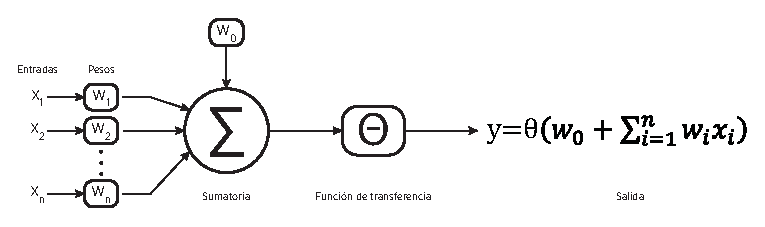
\includegraphics[width=0.65\textwidth]{imagenes/rna}
	\caption{Modelo perceptrón}
	\label{fig:perceptron-rna}
\end{figure*}

El proceso de entrenamiento de una neurona o una RBA consiste en encontrar los pesos $w_0, \cdots, w_n$ a través de un algoritmo de aprendizaje para capturar el conocimiento, tal que:
\begin{equation}
	w_i = \sum_{j=1}^m y_j x_j^i,~~~ \forall i = 1,2,\cdots,n
\end{equation}
donde $m$ es el número de muestras de aprendizaje, $y_j$ es la salida deseada del vector de patrón $x_j$ y $x_j^i$ es la $i$-ésima dimensión del patrón de entrada.

A pesar de la formalidad matemática ofrecida por el modelo perceptrón, éste no era capaz de representar una operación \emph{XOR} y en general cualquier problema en el que no existiera separación lineal entre las clases.

Un paso hacia la solución de los problemas linealmente no separables fue la adición de una capa de pesos oculta al modelo perceptrón.
Sin embargo, aunque el modelo expandido con capas ocultas en teoría ofrecía solución a los problemas, no existía un algoritmo para realizar el entrenamiento y cálculo de los pesos en cada una de ellas.

Fue hasta 1986 cuando Rumelhart propuso el algoritmo retro-propagación del error para realizar el entrenamiento de las redes.
Este algoritmo se encuentra basado en el método de descenso de gradiente para minimizar el error y es ampliamente utilizado para el entrenamiento supervisado de las RNA.

Una RNA multicapa (o MLP, Multilayer Perceptron) puede ser entendida tal como se muestra en la Figura \ref{fig:rna-mlp}.
Cada una de las neuronas es excitada por las entradas y en conjunto con los pesos se evalúan dentro de una función de transferencia para otorgar una salida excitatoria o inhibitoria hacia el resto de las neuronas con las que se encuentra conectada.
Existen muchas funciones de transferencia, una de las más utilizadas es la función sigmoidal debido a la sencillez para calcular su derivada.
Los siguientes párrafos describen los procesos de entrenamiento y clasificación en las RNA MLP.
\begin{figure}[tb]
	\centering
	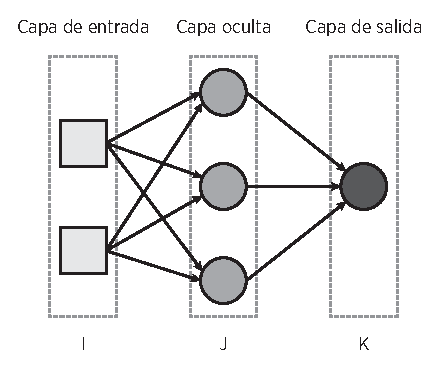
\includegraphics[scale=0.75]{imagenes/mlp}
	\caption{RNA multicapa}
	\label{fig:rna-mlp}
\end{figure}

\subsection{Entrenamiento de una RNA} % (fold)
\label{sub:entrenamiento_de_una_RNA}
El entrenamiento de una RNA requiere definir los siguientes elementos:
\begin{itemize}
	\item \textbf{Algoritmo de aprendizaje}: Indica cómo actualizar los pesos para obtener un mínimo de errores.
	\item \textbf{Regla de aprendizaje}: Indica cómo un peso es actualizado si existe un error.
	\item \textbf{Conjunto de aprendizaje}: Son las $m$ muestras de aprendizaje.
	\item Muestra de aprendizaje: Es un vector de $n$ elementos, $x_1, \cdots, x_n$ con la salida deseada. 
\end{itemize}


De estos elementos se desprende que el entrenamiento de una RNA multicapa consiste en el cálculo de los mejores valores para los pesos de cada neurona en cada una de las capas.

\subsubsection{Cálculo del error} % (fold)
\label{ssub:c_lculo_del_error}

% subsubsection c_lculo_del_error (end)
El conocer los \emph{mejores} pesos se encuentra relacionado con los errores o discrepancias entre la salida de la RNA y las etiquetas reales.

El error puede ser calculado a través de:
$$
E=\frac{1}{2} \sum_{k\in K}(O_k - t_k)^2
$$

donde $t_j$ es la salida deseada del nodo $j$ en la capa de salida y $O_k$ es la salida de los nodos en la capa $k$ (de salida).
Evidentemente, para minimizar el error se debe calcular $\frac{\partial E}{\partial W_{jk}^l}$, que se refiere a la derivada del error respecto a los pesos en cada una de las capas.
Es por ello que se reliza una distinción de si el nodo se encuentra en la capa de salida o en la capa oculta.

Para un nodo en la capa de salida:
$$
\frac{\partial E}{\partial W_{jk}} = \delta_k O_j
$$
donde $\delta _k = (O_k - t_k) O_k (1 - O_k)$


Para un nodo en la capa oculta (considerando una RNA de únicamente tres capas):
$$
\frac{\partial E}{\partial W_{ij}} = \delta_j O_i
$$
donde $\delta _j = O_j (1 - O_j) \sum_{k \in K}\delta _k W_{jk}$

Para el caso de las RNA, el valor del bias permite desplazar el hiperplano de decisión para obtener un mejor ajuste.
Su cálculo implica el agregar una entrada ficticia con valor de 1 para cada una de las neuronas, de tal manera que los pesos bias se actualizan igual que los pesos sinápticos en cada iteración.

\subsubsection{Cálculo de los pesos} % (fold)
\label{ssub:c_lculo_de_los_pesos}
Como ha sido mencionado, el algoritmo de back-propagation permite realizar el entrenamiento de la RNA.
Este algoritmo está basado en el método del descenso del gradiente, por ello el cálculo del error resulta de utilidad ya que permite realizar la adaptación de los valores de los pesos de acuerdo a su variación.

El algoritmo de \emph{back-propagation} es mostrado en Pseudocódigo \ref{alg:algoritmo-entrenamiento}.
Es preciso notar que existe una primera etapa de \emph{Feed-forward} en la que se va alimentando a la red hacia adelante en cada una de las capas, calculando las discrepancias entre sus salidas y la salida esperada.
Posteriormente, la etapa de \emph{back-propagation} actualiza los pesos, indicada en la línea \ref{alg:actualizacion-pesos}, muestra cómo se emplean los errores y los resultados de la iteración anterior para la actualización de los pesos yendo de la última capa a la inicial.

\begin{algorithm} 
\footnotesize
\begin{algorithmic}[1] 
\REQUIRE  $x$, $y$, $\eta$ $\alpha$, $e_min$, $t_max$
\ENSURE $W_{ij}$, $W_{jk}$
\STATE Inicializar aleatoriamente los pesos $W_{ij},~W_{jk}$
\STATE $t=0$
\REPEAT
\STATE \emph{Feed-forward} Calcular salida de la red $O_k$ con los datos de entrada
\STATE Calcular $\delta _k$ para cada nodo de la capa de salida
\STATE Calcular $\delta _j$ para cada nodo de la capa oculta
\STATE Actualizar pesos de cada capa $l$ mediante \emph{back-propagation}:
$$W_l(t+1) = W_l(t)+\Delta W_l(t) + \alpha W_l (t-1)$$ \label{alg:actualizacion-pesos}
donde $$\Delta W_l (t) = \eta \delta _l O_{l-1}$$
\STATE $t = t + 1$
\UNTIL {$\text{MeanSquareError}(y-O_k) < e_{min} ~\mathbf{o}~ (t=t_{max})$}
\RETURN $W_{ij}$, $W_{jk}$
\end{algorithmic} 
\caption{Algoritmo de entrenamiento} 
\label{alg:algoritmo-entrenamiento}
\end{algorithm}


\subsection{Clasificación en una RNA} % (fold)
\label{sub:clasificaci_n_en_una_rna}
Una vez que se ha realizado el entrenamiento de la RNA, el proceso de clasificación es implementado al especificar como entrada de la RNA los datos que se desea clasificar para desencadenar la etapa de \emph{Feed forward}.
Por lo tanto, el proceso de clasificación es meramente calcular la salida $O_k$ a partir de los datos de prueba, como se muestra en el Pseudocódigo \ref{alg:algoritmo-clasificacion}.

\begin{algorithm} 
\footnotesize
\begin{algorithmic}[1] 
\REQUIRE  $X$, $Y$, $W_{ij}$, $W_{jk}$
\ENSURE $Y_p$, $\text{error}$
\STATE $N=\text{Muestras en X}$:
\STATE Salida en capa oculta:
\STATE $V = W_{ij} * X$
\STATE $S = \Theta (V)$ (Función de transferencia), específicamente: $S = \frac{1}{1 + \text{exp}(-V)}$

\STATE Salida en capa de salida:
\STATE $G = W_{jk} * S$
\STATE $O = \Theta (G)$ (Función de transferencia), específicamente: $S = \frac{1}{1 + \text{exp}(-G)}$
\STATE $Y_{p_i} = O_i > 0.5? 1 : 0, ~\forall i = 1,2,\cdots,N$
\STATE $\text{Err}_i = Y_i - O_i, ~\forall i = 1,2,\cdots,N$
\STATE $\text{error} = \frac{1}{N}(\sum_{i=1}^{N}\text{Err}_i)$
\RETURN $Y_p,\text{error}$
\end{algorithmic} 
\caption{Algoritmo de clasificacion} 
\label{alg:algoritmo-clasificacion}
\end{algorithm}

\section{Metodología}
\label{sec:metodologia}
La metodología seguida se sujetó por completo a las etapas de entrenamiento y clasificación mostradas en el marco teórico de la Sección \ref{sec:marco_teorico}.

Se implementaron dos funciones correspondientes al entrenamiento y la clasificación utilizando \emph{Matlab}.
Con la intención de probar distintas alternativas en la configuración de parámetros se  seleccionó el conjunto de parámetros mostrados en la Tabla \ref{tbl:parametros}, realizando la ejecución de la combinación de todos ellos a manera de malla.
La prueba de cada configuración de parámetros fue probada 31 veces, debido al componente aleatorio existente al permutar los índices de los datos en el entrenamiento.

\begin{table}[h]
\centering
\begin{tabular}{@{}cl@{}}
\toprule
\textbf{Parámetro} & \multicolumn{1}{c}{\textbf{Valores}} \\ \midrule
$H$ (neuronas en capa oculta)                  & 3, 5, 10, 20                         \\
$\eta$                & 0.005 0.01, 0.05, 0.1                \\
$\alpha$             & 1e-7, 5e-7, 1e-6                     \\
$T_{max}$          & 20000                                \\
$E_{min}$          & 1e-9                                 \\ \bottomrule
\end{tabular}
\caption{Configuración de parámetros para la ejecución de la RNA}
\label{tbl:parametros}
\end{table}

En una prueba empírica, se lanzó la ejecución de un conjunto de operaciones de entrenamiento y clasificación, obteniendo 8 segundos en el tiempo de cálculo.
Asumiendo una duración similar en cada configuración, el tiempo esperado de ejecución de toda la actividad se estimó en $\text{longitud}(H) * \text{longitud}(\eta) * \text{longitud}(\alpha) * \text{longitud}(\text{datasets}) * 31 * 8 \text{seg} \approx 793 \text{min} \approx 13 \text{hrs}$.

Debido a este largo tiempo estimado de espera, se decidió hacer adecuaciones en el código para utilizar los ciclos \emph{parfor} provistos por \emph{Matlab} para clasificar cada dataset de forma simultánea.


\section{Resultados} 
\label{sec:resultados}
La experimentación fue realizada en un equipo de cómputo con un procesador Intel core i7 de 8 núcleos a 2.00 GHz con 6 GB de memoria en RAM.

La Tabla \ref{tab:best-rna} muestra un resumen de las mejores ejecuciones para cada uno de los datasets.
La serie de Figuras \cref{fig:espacio-particionado-complex,fig:espacio-particionado-linear,fig:espacio-particionado-ring,fig:espacio-particionado-xor} muestra el espacio particionado obtenido por las mejores configuraciones de parámetros con las que se lanzó la ejecución del entrenamiento y clasificación de las RNA.
Se entiende por \emph{mejor} configuración a aquella que obtuvo el menor error.
Es importante mencionar que se muestra la primera configuración que alcanzó el menor error.

\begin{table}[h]
\centering
\begin{tabular}{@{}cllllll@{}}
\toprule
\textbf{Dataset} & \multicolumn{1}{c}{\textbf{Avg tiempo}} & \multicolumn{1}{c}{\textbf{min MSE}} & \multicolumn{1}{c}{\textbf{Avg MSE}} & \multicolumn{1}{c}{\textbf{$H$}} & \multicolumn{1}{c}{\textbf{$\alpha$}} & \multicolumn{1}{c}{\textbf{$\eta$}} \\ \midrule
complex          & 17.1 segs                               & 0.089109                               & 0.3644                                    & 20                             & 5.00E-07                           & 0.01                            \\
linear           & 12.9 segs                               & 0                                      & 0.1967                                    & 3                              & 1.00E-07                           & 0.005                           \\
ring             & 12.9 segs                               & 0.008                                  & 0.1261                                    & 3                              & 1.00E-07                           & 0.01                            \\
xor              & 6.1 segs                                & 0                                      & 0.0459                                    & 5                              & 1.00E-07                           & 0.005                           \\ \bottomrule
\end{tabular}
\caption{Mejores RNA obtenidas}
\label{tab:best-rna}
\end{table}

\begin{figure}[tb]
	\centering
	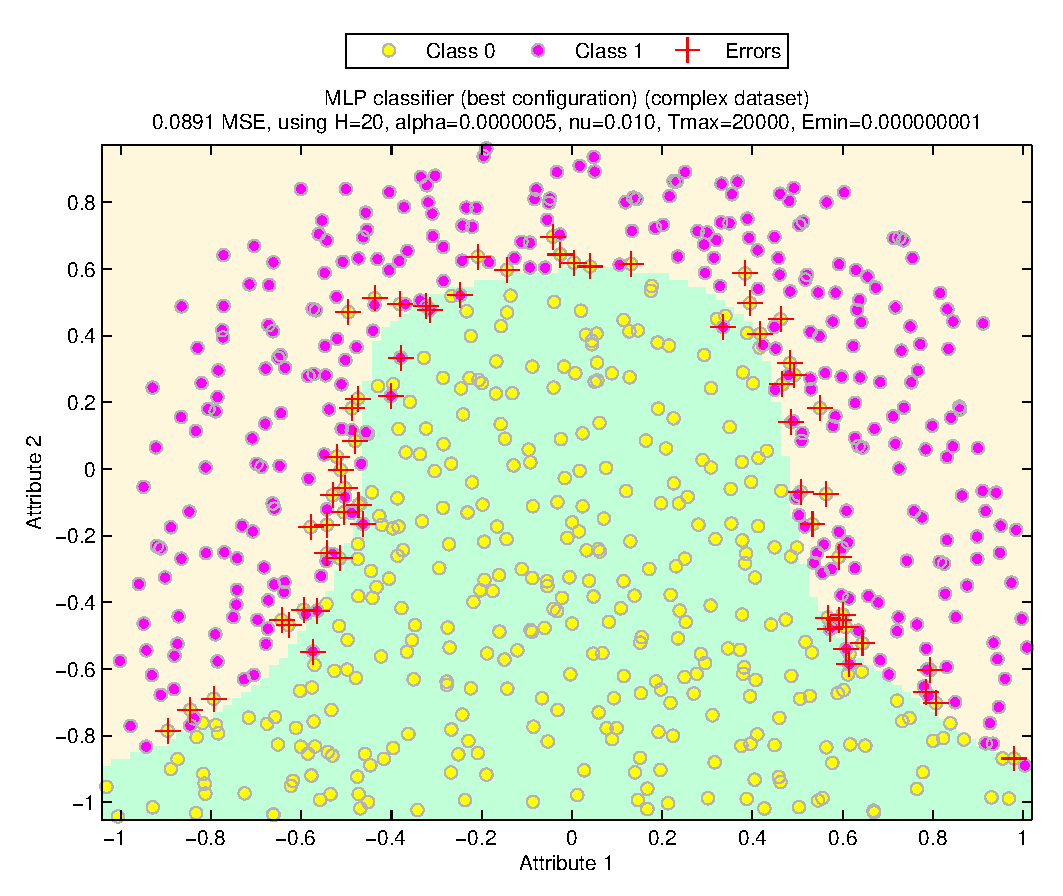
\includegraphics[width=\columnwidth]{imagenes/complex}
	\caption{Espacio particionado de la mejor RNA para el dataset \emph{complex}}
	\label{fig:espacio-particionado-complex}
\end{figure}

\begin{figure}[tb]
	\centering
	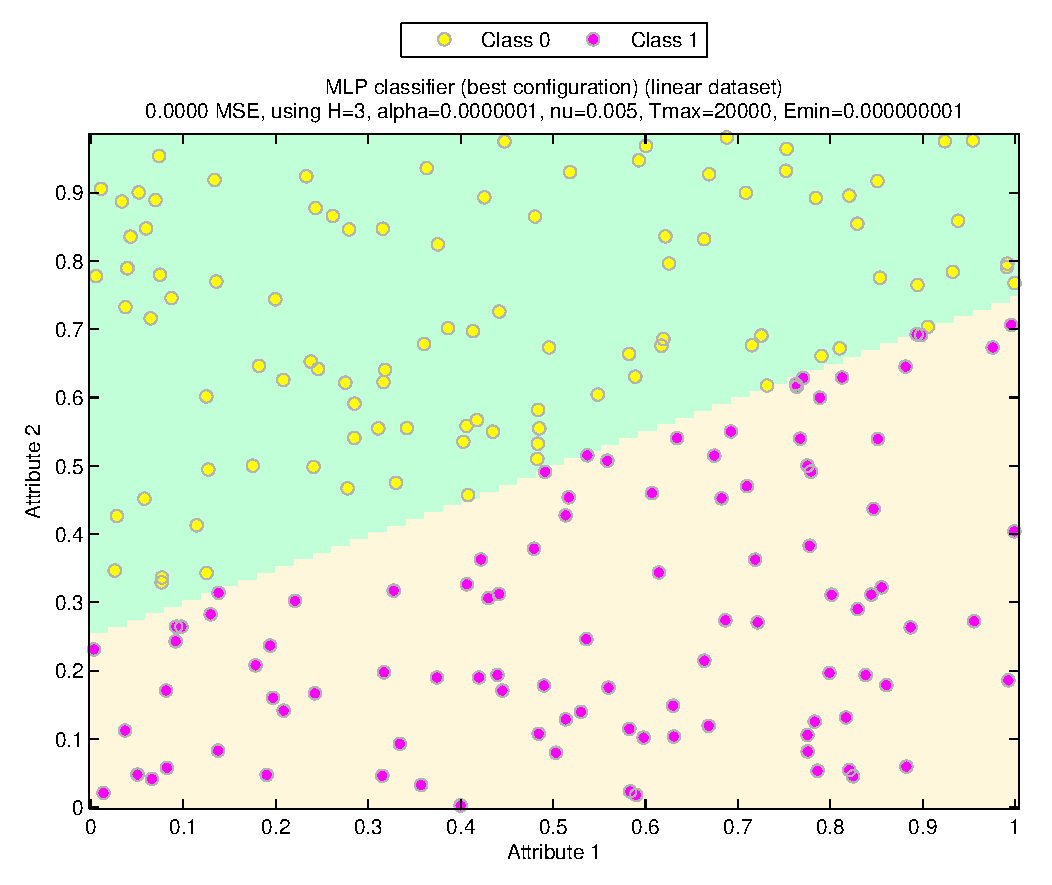
\includegraphics[width=\columnwidth]{imagenes/linear}
	\caption{Espacio particionado de la mejor RNA para el dataset \emph{linear}}
	\label{fig:espacio-particionado-linear}
\end{figure}

\begin{figure}[tb]
	\centering
	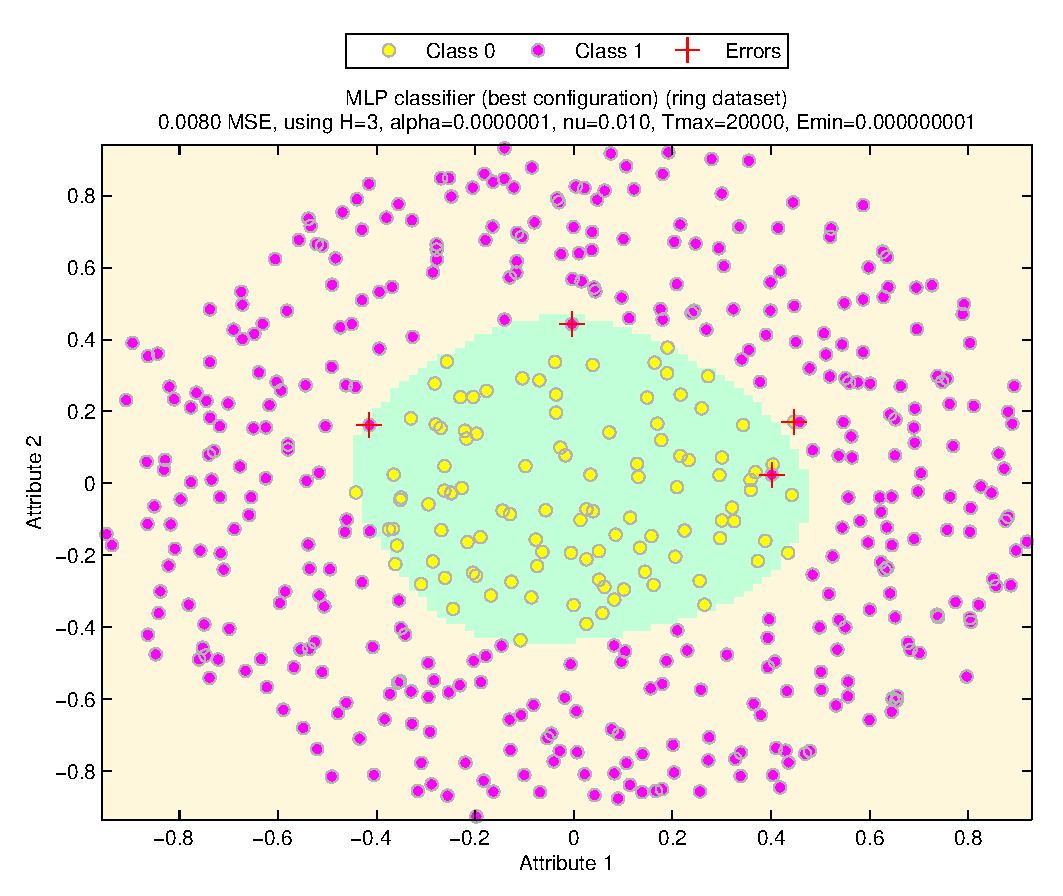
\includegraphics[width=\columnwidth]{imagenes/ring}
	\caption{Espacio particionado de la mejor RNA para el dataset \emph{ring}}
	\label{fig:espacio-particionado-ring}
\end{figure}

\begin{figure}[tb]
	\centering
	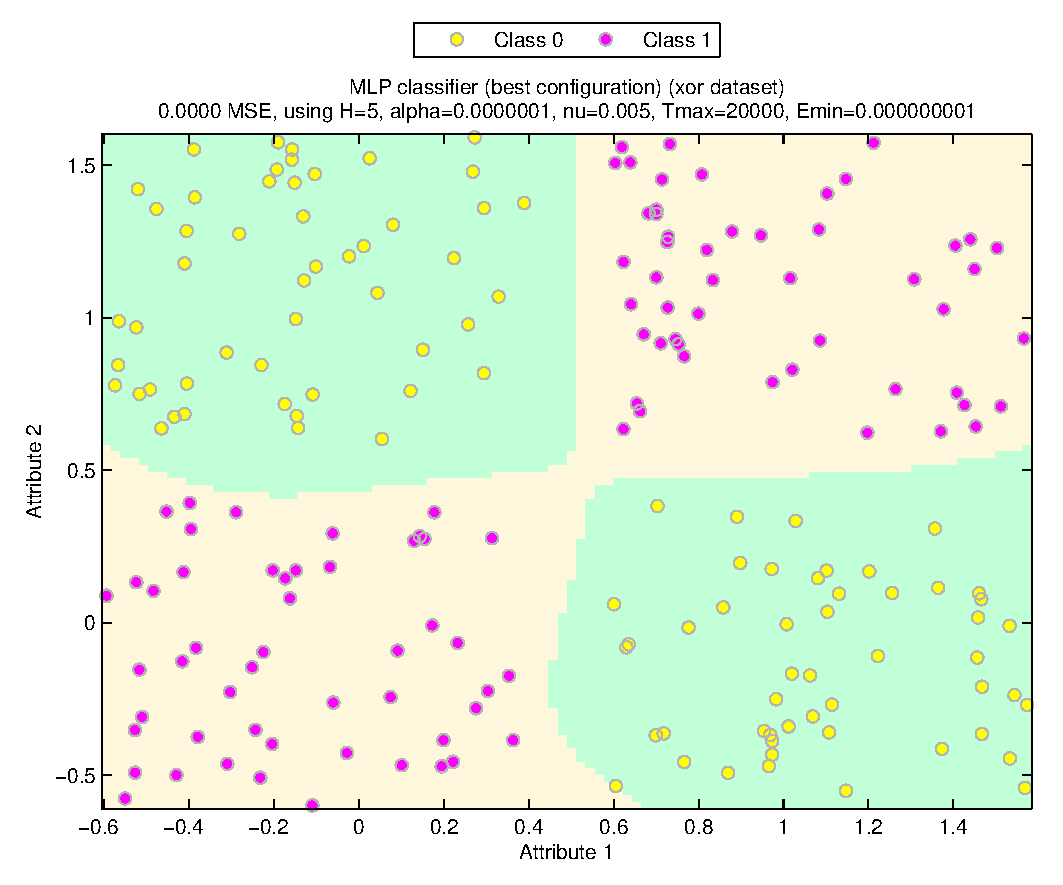
\includegraphics[width=\columnwidth]{imagenes/xor}
	\caption{Espacio particionado de la mejor RNA para el dataset \emph{xor}}
	\label{fig:espacio-particionado-xor}
\end{figure}


\section{Discusión de resultados}
\label{sec:discusion}
Para el caso de los datasets de \emph{linear} y \emph{xor}, las RNA creadas lograron alcanzar una separación perfecta.
Las regiones particionadas de estos datasets (Figura \ref{fig:espacio-particionado-linear} y Figura \ref{fig:espacio-particionado-xor}, respectivamente) demuestran zonas bien definidas, lo cual ayuda a alcanzar porcentajes de error \emph{perfectos} (en $0$).
Adicionalmente, estas separaciones fueron obtenidas con un pequeño número de neuronas, 3 y 5 respectivamente.

El dataset \emph{ring} muestra un grupo de datos formando un anillo y otro grupo de datos al interior de éste (Figura \ref{fig:espacio-particionado-ring}).
Sin embargo, la frontera entre ambos datasets no logra estar perfectamente definida, por lo que se observa un ligero error (alrededor de cuatro patrones mal clasificados).
La mejor RNA para este dataset también requirió apenas 3 neuronas.


Finalmente, el dataset \emph{complex} requirió 20 neuronas en la capa oculta para obtener el menor valor de error (MSE de 0.0891).
El espacio particionado obtenido para este dataset (\ref{fig:espacio-particionado-complex})) muestra una especie de campana con una frontera entre clases que no es linealmente separable a la perfección, por lo que existe una buena cantidad de errores en la clasificación.
Es importante mencionar que este dataset fue el que mayor tiempo requirió para su procesamiento.

De forma general, es posible indicar que las redes neuronales obtienen buenos resultados a la hora de clasificar ya que, según la experimentación mostrada, alcanzan a definir hiperplanos de separación suaves.

Sin embargo, es preciso indicar que no existen lineamientos para la elección de parámetros para su entrenamiento y clasificación.
De hecho, se notó que para el caso del dataset \emph{linear} un fenómeno interesante en el que la mitad de las configuraciones obtuvieron un MSE de $0$, mientras que el resto, de forma intercalada entre las configuraciones \emph{perfectas} obtuvieron errores cada vez más grandes conforme se aumentaba la magnitud de los parámetros.
Para el caso del datase \emph{xor} también se observa una situación peculiar, las últimas configuraciones con 20 neuronas obtienen un 50\% de error, a pesar del hecho de contar con el mayor número de neuronas.
El punto de esta idea es que la elección de parámetros es difícil para este tipo de técnica.


\section{Conclusiones}
\label{sec:conclusiones}
Las redes neuronales intentan modelar el comportamiento seguido por el cerebro humano al aprender.
Basan su funcionamiento en un elemento que es \emph{excitado} por un conjunto de datos de entrada, que al ser evaluados en una función de transferencia, pueden desencadenar una salida excitatoria o inhibitoria dependiendo de si logran sobrepasar un umbral determinado.

La conexión entre varias neuronas permite potenciar los alcances del perceptrón, sin embargo es preciso encontrar los mejores pesos que serán utilizados por la función de transferencia.
Uno de los métodos para calcular estos pesos en una RNA MLP (una capa de entrada, capas ocultas y capa de salida) es el algoritmo de retro-propagación del error (\emph{back-propagation error}), el cual funciona primero calculando la salida de la red en cada capa considerando los pesos actuales, esto en la etapa de \emph{feed-forward}.
Posteriormente, en la etapa de \emph{back-propagation} el algoritmo actualiza los pesos sinápticos, considerando la discrepancia entre la salida actual y la salida esperada.

El presente documento ha presentado la implementación de una RNA MLP utilizando el algoritmo de \emph{back-propagation}, las regiones particionadas producidas por cada dataset de prueba, así como una discusión de los resultados obtenidos.
En general, se observa que las RNA implementadas obtienen resultados con bajos niveles de error, sin embargo, esto se condiciona debido a la dificultad para elegir la configuración de parámetros adecuada, al no existir lineamientos o \emph{best-practices} para su cálculo.

\nocite{*}
\bibliographystyle{ieeetran}
\bibliography{referencias}


\end{document}

